\section{邻近映射与隐式更新}
\label{sec:opt-ns-prox}

次梯度法每轮只取一条支撑斜率，尖点处其余的形状信息全部丢掉了，这正是它在尖点附近来回跳动的原因。若非光滑函数足够简单，可以换一种做法：不读取它的斜率，而是把它完整地放进一个小的优化子问题，再加一项“不要离当前点太远”的二次惩罚。本节先建立这种子问题的解，即邻近映射，证明它存在唯一、刻画它的最优条件和稳定性；然后计算几类常用函数的邻近映射，其中闭凸集上的投影是一个特例；最后把整个目标放进邻近子问题，得到邻近点法。下一节的复合方法会把这一运算与光滑部分的梯度步组合起来。

\subsection{邻近映射的定义与性质}
\label{sec:opt-ns-prox-def}

给定中心$\bm z$和函数$r$，考虑子问题
\[
 \min_{\bm x}\ r(\bm x)+\frac1{2\eta}\lVert\bm x-\bm z\rVert_2^2 .
\]
只最小化$r$，解可能离$\bm z$很远，甚至不存在；只最小化距离项，解就是$\bm z$本身，$r$没有得到任何改善。二者相加，参数$\eta>0$决定两者的相对分量：$\eta$小时距离项占主导，解贴近$\bm z$；$\eta$大时$r$的作用增强。

图~\ref{fig:opt-ns-prox-subproblem}在$r(w)=|w|$、$\eta=1$下画出两个中心对应的子问题。可以把它想成一根连在$z$上的弹簧拉着点$w$，弹簧的拉力是$(z-w)/\eta$；而$|w|$像一块有摩擦的地面，在$w\neq0$时始终以大小为$1$的力把$w$推向原点，在$w=0$处则能提供$[-1,1]$中任意大小的阻力。$z=0.5$时，弹簧在原点的拉力只有$0.5$，摩擦挡得住，解停在$0$；$z=2$时，弹簧把点拉到$w=1$，此时拉力$1$恰好与摩擦力平衡。这个类比对应的正是下面的最优条件$(\bm z-\bm p)/\eta\in\partial r(\bm p)$：拉力必须是$r$在解处的某条次梯度。

\begin{figure}[!htbp]
  \centering
  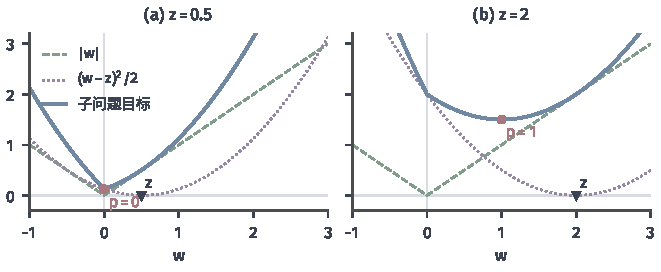
\includegraphics[width=112mm]{figures/03-optimization-evolution-and-signals/01-optimization/matplotlib/c4-prox-subproblem/figure.pdf}
  \caption{邻近子问题$|w|+(w-z)^2/2$（$\eta=1$）。绿色虚线是非光滑项$|w|$，紫色点线是以中心$z$（黑色三角）为最低点的二次距离项，蓝线是两者之和，红点是子问题的最小点$p$。(a) $z=0.5$时$p=0$：在原点处$z-p=0.5$落在$\partial|\cdot|(0)=[-1,1]$中。(b) $z=2$时$p=1$：$z-p=1$恰等于$|\cdot|$在$1$处的斜率。}
  \label{fig:opt-ns-prox-subproblem}
\end{figure}

要让这个子问题对任何中心都有唯一的解，需要对$r$提出条件。回顾第~\ref{chap:optimization}章：$r$下半连续，是指$\bm x_k\to\bm x$时总有$r(\bm x)\leq\liminf_kr(\bm x_k)$；下半连续函数若有非空的紧下水平集，就能取得最小值。

\begin{definition}[邻近映射]
\label{def:opt-ns-prox}
设$r:\mathbb R^d\to\mathbb R\cup\{+\infty\}$是适当、下半连续的凸函数，$\eta>0$。对每个$\bm z\in\mathbb R^d$，令
\begin{equation}
 \operatorname{prox}_{\eta r}(\bm z)=\argmin_{\bm x\in\mathbb R^d}\Bigl\{r(\bm x)+\frac1{2\eta}\lVert\bm x-\bm z\rVert_2^2\Bigr\},
 \label{eq:opt-ns-prox-def}
\end{equation}
称$\operatorname{prox}_{\eta r}$为$r$（以参数$\eta$）的\term{邻近映射}（proximal mapping），也称\term{邻近算子}（proximal operator）。
\end{definition}

定义中把$\argmin$写成一个点，需要先证明最小点存在且唯一。下面的定理同时给出它的最优条件；证明只用函数值比较，不依赖次微分的求和等式。

\begin{theorem}[邻近映射的存在唯一与最优条件]
\label{thm:opt-ns-prox-characterization}
在定义~\ref{def:opt-ns-prox}的条件下，对每个$\bm z$，子问题~\eqref{eq:opt-ns-prox-def}有唯一最小点$\bm p$。并且对$\bm p\in\operatorname{dom}r$，以下三条等价：
\begin{enumerate}
  \item $\bm p=\operatorname{prox}_{\eta r}(\bm z)$；
  \item $(\bm z-\bm p)/\eta\in\partial r(\bm p)$；
  \item 对所有$\bm y$，$r(\bm y)+\dfrac1{2\eta}\lVert\bm y-\bm z\rVert_2^2\geq r(\bm p)+\dfrac1{2\eta}\lVert\bm p-\bm z\rVert_2^2+\dfrac1{2\eta}\lVert\bm y-\bm p\rVert_2^2$。
\end{enumerate}
\end{theorem}

\begin{proof}
\emph{存在。}记子问题目标为$\phi(\bm x)=r(\bm x)+\lVert\bm x-\bm z\rVert_2^2/(2\eta)$。先说明$r$至多以线性速度向$-\infty$下降。取$\bm x_0\in\operatorname{dom}r$。$r$下半连续，在紧集$\{\bm x:\lVert\bm x-\bm x_0\rVert_2\leq1\}$上取得最小值$m$，$m$有限且$m\leq r(\bm x_0)$。对$\lVert\bm x-\bm x_0\rVert_2>1$，令$\theta=1/\lVert\bm x-\bm x_0\rVert_2$，点$\bm u=(1-\theta)\bm x_0+\theta\bm x$在这个单位球面上，凸性给出$m\leq r(\bm u)\leq(1-\theta)r(\bm x_0)+\theta r(\bm x)$，整理得
\[
 r(\bm x)\geq r(\bm x_0)-\bigl(r(\bm x_0)-m\bigr)\lVert\bm x-\bm x_0\rVert_2 .
\]
因此$\phi(\bm x)\geq r(\bm x_0)-c\lVert\bm x-\bm x_0\rVert_2+\lVert\bm x-\bm z\rVert_2^2/(2\eta)$，其中$c=r(\bm x_0)-m\geq0$。二次项最终压过线性项，$\phi$的每个下水平集都有界；$\phi$下半连续，所以下水平集是闭集，从而是紧集。$\phi(\bm x_0)<+\infty$保证下水平集$\{\phi\leq\phi(\bm x_0)\}$非空，由第~\ref{chap:optimization}章的存在性结论，最小点存在。

\emph{(1)$\Rightarrow$(2)。}设$\bm p$是最小点，任取$\bm y$与$\theta\in(0,1)$，令$\bm p_\theta=\bm p+\theta(\bm y-\bm p)$。由最小性和$r$的凸性，
\[
 \begin{aligned}
 r(\bm p)+\frac{\lVert\bm p-\bm z\rVert_2^2}{2\eta}
 &\leq r(\bm p_\theta)+\frac{\lVert\bm p_\theta-\bm z\rVert_2^2}{2\eta}\\
 &\leq(1-\theta)r(\bm p)+\theta r(\bm y)+\frac{\lVert\bm p-\bm z\rVert_2^2}{2\eta}\\
 &\qquad+\frac\theta\eta\langle\bm p-\bm z,\bm y-\bm p\rangle+\frac{\theta^2}{2\eta}\lVert\bm y-\bm p\rVert_2^2.
 \end{aligned}
\]
消去相同项、除以$\theta$，再令$\theta\downarrow0$，得$r(\bm y)\geq r(\bm p)+\langle(\bm z-\bm p)/\eta,\bm y-\bm p\rangle$，这正是(2)。

\emph{(2)$\Rightarrow$(3)。}由(2)，$r(\bm y)\geq r(\bm p)+\frac1\eta\langle\bm z-\bm p,\bm y-\bm p\rangle$。再利用恒等式
\[
 \lVert\bm y-\bm z\rVert_2^2=\lVert\bm y-\bm p\rVert_2^2+2\langle\bm y-\bm p,\bm p-\bm z\rangle+\lVert\bm p-\bm z\rVert_2^2,
\]
两式相加后内积项恰好抵消，即得(3)。

\emph{(3)$\Rightarrow$(1)与唯一性。}(3)说明$\phi(\bm y)\geq\phi(\bm p)+\lVert\bm y-\bm p\rVert_2^2/(2\eta)$，所以$\bm p$是最小点，并且任何$\bm y\neq\bm p$的目标值都严格更大，最小点唯一。
\end{proof}

条件(2)可以读成一个隐式的次梯度步：$\bm p=\bm z-\eta\bm g$，其中$\bm g\in\partial r(\bm p)$。与次梯度法的显式步$\bm z-\eta\bm g$、$\bm g\in\partial r(\bm z)$相比，斜率是在新点而不是旧点读取的。条件(3)比最小性更强：解的目标值比任何其他候选至少低一个二次量，后面分析邻近梯度法和邻近点法时都要用它。

\paragraph{子问题的解不是原问题的解}
$\operatorname{prox}_{\eta r}(\bm z)$是一个强凸子问题的解，一般不是$r$本身的最小点。在图~\ref{fig:opt-ns-prox-subproblem}(b)中，$|w|$的最小点是$0$，子问题的解却是$1$。两者重合的情形可以准确刻画：由条件(2)，$\operatorname{prox}_{\eta r}(\bm z)=\bm z$当且仅当$\bm 0\in\partial r(\bm z)$，即$\bm z$是$r$的最小点。邻近映射的不动点恰好是原函数的最小点；这就是后面用反复调用邻近映射去求最小点的依据。

\paragraph{非扩张性}
设$\bm p_1=\operatorname{prox}_{\eta r}(\bm z_1)$，$\bm p_2=\operatorname{prox}_{\eta r}(\bm z_2)$。把条件(2)的支撑不等式分别用于对方的点：
\[
 r(\bm p_2)\geq r(\bm p_1)+\tfrac1\eta\langle\bm z_1-\bm p_1,\bm p_2-\bm p_1\rangle,\qquad
 r(\bm p_1)\geq r(\bm p_2)+\tfrac1\eta\langle\bm z_2-\bm p_2,\bm p_1-\bm p_2\rangle.
\]
两式相加，$r$的值抵消，得$\langle(\bm z_1-\bm z_2)-(\bm p_1-\bm p_2),\bm p_1-\bm p_2\rangle\geq0$，即
\begin{equation}
 \lVert\bm p_1-\bm p_2\rVert_2^2\leq\langle\bm z_1-\bm z_2,\bm p_1-\bm p_2\rangle\leq\lVert\bm z_1-\bm z_2\rVert_2\lVert\bm p_1-\bm p_2\rVert_2 .
 \label{eq:opt-ns-prox-firm}
\end{equation}
所以$\lVert\operatorname{prox}_{\eta r}(\bm z_1)-\operatorname{prox}_{\eta r}(\bm z_2)\rVert_2\leq\lVert\bm z_1-\bm z_2\rVert_2$：邻近映射是\term{非扩张映射}（nonexpansive mapping），中心的误差不会在一次调用中被放大。在迭代算法里，中心往往由带误差的梯度算出，这一性质保证一次邻近调用不会额外放大这个误差。

\paragraph{可解不等于便宜}
定理~\ref{thm:opt-ns-prox-characterization}只说明解存在唯一，没有说明它好算。对一般的$r$，求邻近映射本身就是一个与原问题难度相当的优化问题。邻近方法真正有用，是在$r$有闭式或可快速计算的邻近映射时，下一小节给出几类这样的函数。

\paragraph{弱凸函数的邻近映射}
若$r$不凸但是$\rho$弱凸，并且$0<\eta<1/\rho$，子问题目标$r+\frac1{2\eta}\lVert\cdot-\bm z\rVert_2^2$等于凸函数$r+\frac\rho2\lVert\cdot\rVert_2^2$加上一个系数为$\frac1{2\eta}-\frac\rho2>0$的二次函数，仍然强凸，解存在唯一。但非扩张性不再成立。取$r(x)=-\rho x^2/2$，子问题$-\rho x^2/2+(x-z)^2/(2\eta)$的驻点满足$-\rho x+(x-z)/\eta=0$，解为$\operatorname{prox}_{\eta r}(z)=z/(1-\eta\rho)$，它把中心的差放大了$1/(1-\eta\rho)>1$倍。弱凸推广因此必须限制参数$\eta$，并单独分析误差传播。

\subsection{邻近映射的计算}
\label{sec:opt-ns-prox-computation}

邻近方法的效率取决于邻近映射能否快速计算。本小节先推导$\ell_1$范数的软阈值并与二次正则对照，再把闭凸集的指示函数代入定义，得到投影及其性质。

\paragraph{软阈值}
取$r(\bm x)=\lambda\lVert\bm x\rVert_1$，$\lambda\geq0$。子问题目标$\sum_j\bigl(\lambda|x_j|+(x_j-z_j)^2/(2\eta)\bigr)$逐坐标分离，各坐标可以分别最小化。对一个坐标，由定理~\ref{thm:opt-ns-prox-characterization}的条件(2)，$p$是解当且仅当$(z-p)/\eta\in\lambda\,\partial|\cdot|(p)$。分三种情况：若$p>0$，需$z-p=\eta\lambda$，即$p=z-\eta\lambda$，这要求$z>\eta\lambda$；若$p<0$，同理$p=z+\eta\lambda$，要求$z<-\eta\lambda$；若$p=0$，需$z/\eta\in[-\lambda,\lambda]$，即$|z|\leq\eta\lambda$。三种情况恰好覆盖全部$z$，合起来就是\term{软阈值}（soft thresholding）
\begin{equation}
 \bigl[\operatorname{prox}_{\eta\lambda\lVert\cdot\rVert_1}(\bm z)\bigr]_j=\operatorname{sign}(z_j)\max\{|z_j|-\eta\lambda,0\}.
 \label{eq:opt-ns-soft-threshold}
\end{equation}
例如$\bm z=(3,0.4,-2)^\top$、$\eta\lambda=1$时，输出为$(2,0,-1)^\top$：大的坐标向原点平移$1$，小于阈值的坐标被精确置零。

把它与二次正则对照。$r(\bm x)=\frac\lambda2\lVert\bm x\rVert_2^2$可微，条件(2)化为$\bm z-\bm p=\eta\lambda\bm p$，解为$\bm p=\bm z/(1+\eta\lambda)$；同一输入得$(1.5,0.2,-1)^\top$。二次正则按比例收缩，任何非零坐标都不会变成零；$\ell_1$正则的零区间来自原点处次微分是整段区间：只要中心的拉力不超过阈值，解就停在零。图~\ref{fig:opt-ns-prox-maps}把两种映射与下面的区间投影画在同一坐标系中。

\begin{figure}[!htbp]
  \centering
  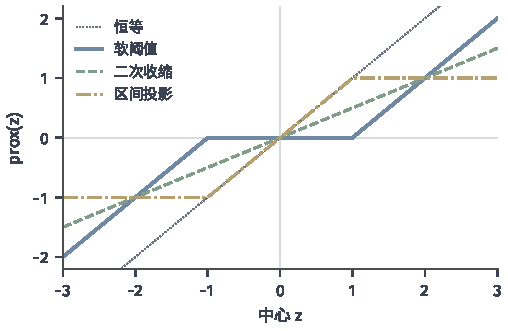
\includegraphics[width=86mm]{figures/03-optimization-evolution-and-signals/01-optimization/matplotlib/c4-prox-maps/figure.pdf}
  \caption{三种一维邻近映射（参数取$1$）。蓝线是$|w|$的软阈值$\operatorname{sign}(z)\max\{|z|-1,0\}$，在$[-1,1]$上恒为零；绿色虚线是$w^2/2$的二次收缩$z/2$，只在$z=0$处为零；黄色点划线是区间$[-1,1]$指示函数的邻近映射，即把$z$截断到区间内；灰色点线是恒等映射。三者都是非扩张的：曲线斜率不超过$1$。}
  \label{fig:opt-ns-prox-maps}
\end{figure}

\paragraph{加权与分组的阈值}
阈值来自原点处次微分的形状，换用别的范数时要重新核验。加权$\ell_1$范数$\sum_j\lambda_j|x_j|$仍然逐坐标分离，各坐标的阈值变为$\eta\lambda_j$。欧氏范数$r(\bm x)=\lambda\lVert\bm x\rVert_2$则不再分离：若$\bm p\neq\bm 0$，条件(2)要求$\bm z-\bm p=\eta\lambda\bm p/\lVert\bm p\rVert_2$，所以$\bm p$与$\bm z$同向，$\bm p=(1-\eta\lambda/\lVert\bm z\rVert_2)\bm z$，这要求$\lVert\bm z\rVert_2>\eta\lambda$；若$\bm p=\bm 0$，条件是$\bm z/\eta$属于$\lambda$倍单位球，即$\lVert\bm z\rVert_2\leq\eta\lambda$。于是
\[
 \operatorname{prox}_{\eta\lambda\lVert\cdot\rVert_2}(\bm z)=\max\Bigl\{1-\frac{\eta\lambda}{\lVert\bm z\rVert_2},0\Bigr\}\bm z ,
\]
整个向量要么一起置零、要么一起沿原方向缩短。对$\bm z=(3,4)^\top$、$\eta\lambda=1$，结果是$(2.4,3.2)^\top$；逐坐标软阈值却给出$(2,3)^\top$，两者不同。

\paragraph{投影}
约束$\bm x\in C$用指示函数$\iota_C$写入目标。设$C$是非空闭凸集，则$\iota_C$适当（$C$非空）、凸（$C$凸）、下半连续（$C$闭），满足定义~\ref{def:opt-ns-prox}的条件。代入定义，
\[
 \operatorname{prox}_{\eta\iota_C}(\bm z)=\argmin_{\bm x\in C}\frac1{2\eta}\lVert\bm x-\bm z\rVert_2^2=\argmin_{\bm x\in C}\lVert\bm x-\bm z\rVert_2 ,
\]
它与$\eta$无关，就是$C$中离$\bm z$最近的点，称为$\bm z$在$C$上的\term{投影}（projection），记为$\Pi_C(\bm z)$。定理~\ref{thm:opt-ns-prox-characterization}和非扩张性直接给出投影的基本性质。

\begin{theorem}[闭凸集上的投影]
\label{thm:opt-ns-projection}
设$C\subseteq\mathbb R^d$是非空闭凸集。则对每个$\bm z$，最近点$\bm p=\Pi_C(\bm z)$存在且唯一，并且$\bm p\in C$由下面的\term{变分不等式}（variational inequality）刻画：
\begin{equation}
 \langle\bm z-\bm p,\bm y-\bm p\rangle\leq0\quad\text{对所有}\ \bm y\in C.
 \label{eq:opt-ns-projection-vi}
\end{equation}
此外，对所有$\bm y\in C$有$\lVert\bm p-\bm y\rVert_2^2+\lVert\bm z-\bm p\rVert_2^2\leq\lVert\bm z-\bm y\rVert_2^2$，并且$\lVert\Pi_C(\bm z_1)-\Pi_C(\bm z_2)\rVert_2\leq\lVert\bm z_1-\bm z_2\rVert_2$。
\end{theorem}

\begin{proof}
存在唯一与非扩张性是定理~\ref{thm:opt-ns-prox-characterization}和式~\eqref{eq:opt-ns-prox-firm}在$r=\iota_C$时的特例。条件(2)写成$\iota_C(\bm y)\geq\iota_C(\bm p)+\frac1\eta\langle\bm z-\bm p,\bm y-\bm p\rangle$对所有$\bm y$成立；$\bm y\notin C$时左端为$+\infty$，自动成立，$\bm y\in C$时它就是式~\eqref{eq:opt-ns-projection-vi}。条件(3)取$\bm y\in C$、乘以$2\eta$，即得距离不等式。
\end{proof}

式~\eqref{eq:opt-ns-projection-vi}的几何意义是：从投影点$\bm p$指向原点$\bm z$的向量，与从$\bm p$指向$C$中任一点的向量夹角不小于直角。集合$\{\bm v:\langle\bm v,\bm y-\bm p\rangle\leq0\ \text{对所有}\ \bm y\in C\}$是一个闭凸锥，称为$C$在$\bm p$处的\term{法锥}（normal cone），记为$N_C(\bm p)$；它恰好就是$\partial\iota_C(\bm p)$。于是投影的最优条件可以说成：$\bm z-\Pi_C(\bm z)\in N_C(\Pi_C(\bm z))$，即“$\bm z$减去投影点后的残差必须沿法向”。在$C$的内点处法锥只有零向量，所以内点的投影只能是它自己；在光滑边界上法锥是一条外法线射线；在角点处法锥张成一个楔形区域。

\begin{example}[正方形上的投影]
\label{ex:opt-ns-box-projection}
取$C=[0,1]^2$。它的指示函数是两个区间指示函数之和，逐坐标分离，所以投影就是逐坐标截断：$[\Pi_C(\bm z)]_j=\min\{\max\{z_j,0\},1\}$。对$\bm z_a=(1.6,0.6)^\top$，投影$\bm p_a=(1,0.6)^\top$落在右边上，残差$(0.6,0)^\top$沿该边的外法线；对$C$中任一点$\bm y$，$\langle\bm z_a-\bm p_a,\bm y-\bm p_a\rangle=0.6(y_1-1)\leq0$。对$\bm z_b=(1.7,-0.5)^\top$，投影是顶点$\bm p_b=(1,0)^\top$，残差$(0.7,-0.5)^\top$；该顶点的法锥是$\{\bm v:v_1\geq0,\ v_2\leq0\}$，残差确实在其中。图~\ref{fig:opt-ns-projection}画出了这两种情形。
\end{example}

\begin{figure}[!htbp]
  \centering
  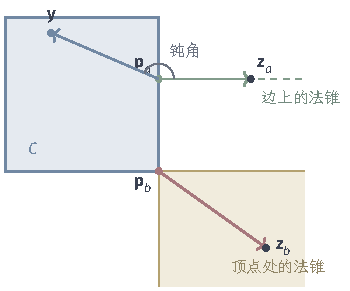
\includegraphics[width=59.33mm]{figures/03-optimization-evolution-and-signals/01-optimization/tikz/c4-projection-normal-cone/figure.pdf}
  \caption{正方形$C=[0,1]^2$上的投影与法锥。$\bm z_a=(1.6,0.6)^\top$投影到边上的$\bm p_a=(1,0.6)^\top$，法锥是向右的射线（绿色虚线），残差$\bm z_a-\bm p_a$（绿箭头）与指向$C$中任一点$\bm y$的向量（蓝箭头）成钝角。$\bm z_b=(1.7,-0.5)^\top$投影到顶点$\bm p_b=(1,0)^\top$，该点的法锥是黄色象限，残差$\bm z_b-\bm p_b$（红箭头）落在其中。}
  \label{fig:opt-ns-projection}
\end{figure}

盒约束、球约束（$\Pi(\bm z)=\bm z/\max\{1,\lVert\bm z\rVert_2/\rho\}$对半径$\rho$的球）的投影都有闭式。概率单纯形等约束则不能逐坐标截断，需要专门的计算；这些具体集合的投影及以它们为基础的约束算法在第~\ref{chap:constrained-optimization}章展开，那里直接调用本小节的存在唯一、变分不等式和非扩张性。

\paragraph{不可分的复合项}
可分性是逐坐标公式成立的前提。两项之和的邻近映射一般也不能由两项各自的邻近映射拼出来。以$r(\bm x)=|x_1-x_2|$为例，它惩罚两个坐标之差。由复合规则，$\partial r(\bm p)=\{u(1,-1)^\top:u\in\partial|\cdot|(p_1-p_2)\}$；条件(2)给出$\bm p=\bm z-\eta u(1,-1)^\top$，于是$p_1-p_2=(z_1-z_2)-2\eta u$。若$|z_1-z_2|>2\eta$，取$u=\operatorname{sign}(z_1-z_2)$，两个坐标各向对方移动$\eta$；若$|z_1-z_2|\leq2\eta$，取$u=(z_1-z_2)/(2\eta)$，两个坐标合并为它们的平均值。例如$\eta=1$、$\bm z=(3,0)^\top$时解为$(2,1)^\top$，$\bm z=(1,0)^\top$时解为$(0.5,0.5)^\top$。这里作用的对象是坐标之差，任何逐坐标的阈值规则都得不到这个结果。

\subsection{邻近点法}
\label{sec:opt-ns-proximal-point}

邻近映射的不动点就是最小点。最直接的利用方式，是对整个目标$f$反复调用它的邻近映射。

\paragraph{隐式更新}
设$f$适当、下半连续、凸。\term{邻近点法}（proximal point method）从$\bm x^{(0)}$出发，按
\begin{equation}
 \bm x^{(t+1)}=\operatorname{prox}_{\eta f}(\bm x^{(t)})
 \label{eq:opt-ns-proximal-point}
\end{equation}
迭代。由定理~\ref{thm:opt-ns-prox-characterization}的条件(2)，$\bm x^{(t+1)}=\bm x^{(t)}-\eta\bm g^{(t+1)}$，其中$\bm g^{(t+1)}\in\partial f(\bm x^{(t+1)})$：这是一个次梯度步，但斜率取在尚未知道的新点上，所以称为隐式更新。每轮要做的是固定旧点，组装子问题$f(\bm x)+\lVert\bm x-\bm x^{(t)}\rVert_2^2/(2\eta)$，求出它的最小点。

\paragraph{每轮的下降}
旧点本身是子问题的一个候选，所以子问题最小值不超过旧点处的值$f(\bm x^{(t)})$：
\begin{equation}
 f(\bm x^{(t+1)})+\frac1{2\eta}\lVert\bm x^{(t+1)}-\bm x^{(t)}\rVert_2^2\leq f(\bm x^{(t)}).
 \label{eq:opt-ns-proximal-point-descent}
\end{equation}
与次梯度法不同，邻近点法的目标值逐轮不增，而且每次移动都以位移平方为代价换得下降。这一结论对任何$\eta>0$成立，不需要光滑常数来限制步长。

\begin{example}[绝对值上的两种更新]
\label{ex:opt-ns-proximal-point-abs}
对$f(x)=|x|$、$\eta=1$，邻近点法的每一步就是阈值为$1$的软阈值。从$x^{(0)}=2.5$出发，迭代为$2.5,\ 1.5,\ 0.5,\ 0,\ 0,\dots$，第三步精确到达最小点并停住。同样从$2.5$出发，步长为$1$的次梯度法给出$2.5,\ 1.5,\ 0.5,\ -0.5,\ 0.5,\dots$，在尖点两侧永远来回。图~\ref{fig:opt-ns-prox-point}左图画出邻近点法每轮的子问题：每条虚线是$|x|$加上以当前点为中心的二次项，它的最低点就是下一迭代点；到达$0.5$以后，子问题的最低点落在尖点上。
\end{example}

\begin{figure}[!htbp]
  \centering
  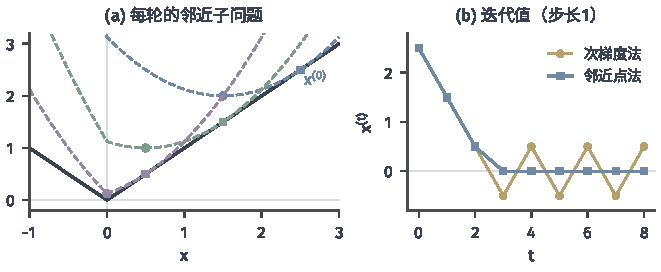
\includegraphics[width=112mm]{figures/03-optimization-evolution-and-signals/01-optimization/matplotlib/c4-prox-point/figure.pdf}
  \caption{邻近点法与次梯度法在$f(x)=|x|$上的比较（$\eta=1$，初值$2.5$）。(a) 黑线是$|x|$；三条虚线是以$x^{(t)}=2.5,1.5,0.5$为中心的子问题$|x|+(x-x^{(t)})^2/2$，方块标出当前点，圆点标出子问题最小点，也就是下一迭代点。(b) 迭代值随$t$的变化：邻近点法第三步到达$0$后停住，次梯度法在$0.5$与$-0.5$之间振荡。}
  \label{fig:opt-ns-prox-point}
\end{figure}

\paragraph{目标差与参数收敛}
下面在凸、最小点存在、子问题精确求解的条件下给出保证。

\begin{theorem}[邻近点法的收敛]
\label{thm:opt-ns-proximal-point}
设$f$适当、下半连续、凸，最小点集合非空，$\eta>0$固定，迭代~\eqref{eq:opt-ns-proximal-point}精确执行。则对任意最小点$\bm x^\star$，距离$\lVert\bm x^{(t)}-\bm x^\star\rVert_2$关于$t$不增，且
\[
 f(\bm x^{(T)})-f^\star\leq\frac{\lVert\bm x^{(0)}-\bm x^\star\rVert_2^2}{2\eta T}.
\]
进一步，整个序列$\bm x^{(t)}$收敛到某个最小点。
\end{theorem}

\begin{proof}
在定理~\ref{thm:opt-ns-prox-characterization}的条件(3)中取$r=f$、$\bm z=\bm x^{(t)}$、$\bm p=\bm x^{(t+1)}$、$\bm y=\bm x^\star$，并略去右端的非负项$\lVert\bm x^{(t+1)}-\bm x^{(t)}\rVert_2^2/(2\eta)$，得
\[
 f(\bm x^{(t+1)})-f^\star\leq\frac1{2\eta}\Bigl(\lVert\bm x^{(t)}-\bm x^\star\rVert_2^2-\lVert\bm x^{(t+1)}-\bm x^\star\rVert_2^2\Bigr).
\]
左端非负，所以距离不增。对$t=0,\dots,T-1$求和，右端相消为不超过$\lVert\bm x^{(0)}-\bm x^\star\rVert_2^2/(2\eta)$；由式~\eqref{eq:opt-ns-proximal-point-descent}，$f(\bm x^{(t)})$不增，左端之和不小于$T\bigl(f(\bm x^{(T)})-f^\star\bigr)$，得到目标差界。

对参数收敛：距离不增说明序列有界，因而有收敛子列$\bm x^{(t_k)}\to\bar{\bm x}$。目标差界说明$f(\bm x^{(t)})\to f^\star$，由下半连续性$f(\bar{\bm x})\leq\liminf_kf(\bm x^{(t_k)})=f^\star$，所以$\bar{\bm x}$是最小点。把距离不增用于$\bm x^\star=\bar{\bm x}$：$\lVert\bm x^{(t)}-\bar{\bm x}\rVert_2$不增，又有一个子列趋于零，故整个序列趋于$\bar{\bm x}$。
\end{proof}

最小点不唯一时，极限是哪一个最小点由初值决定，定理只保证收敛到其中某一个。

\paragraph{代价与不精确求解}
邻近点法没有步长上限，也不需要光滑性，代价转移到了子问题上：每一轮都要精确求解一个与原问题几乎同样困难的强凸问题。例如对最小二乘目标$f(\bm x)=\frac12\lVert\bm A\bm x-\bm b\rVert_2^2$，每轮需要解线性方程组$(\bm A^\top\bm A+\bm I/\eta)\bm x=\bm A^\top\bm b+\bm x^{(t)}/\eta$，代价与直接求解原问题同阶。因此“不受光滑常数限制”不意味着总计算量更少。

实践中子问题只能近似求解。此时必须规定误差标准，例如要求实际输出与精确邻近点的距离不超过预先给定的$\epsilon^{(t)}$，并让这些误差足够快地减小；精确情形的证明不能直接搬用，需要把每轮误差加进上面的不等式重新累计。邻近点法真正的价值在于提供隐式更新的模板：下一节只把目标中简单的那一部分放进邻近子问题，其余部分用梯度近似，从而把每轮子问题变得便宜。
